\section{Superposición coherente entre dos ondas de luz. Interferencia}
\rfigure
%
\pma{
Dos haces de luz linealmente polarizados, con sus campos eléctricos paralelos, se propagan en la misma dirección y sentido. Uno de ellos tiene una intensidad de $\SI{7}{\watt/\metre^2}$ y una frecuencia de 600~THz ($\SI{6E14}{\hertz}$), y el otro una intensidad de $\SI{3}{\watt/\metre^2}$ y una longitud de onda de 500~nm ($\SI{500E-9}{m}$). \textit{a}) Calcule la intensidad resultante si la fase relativa entre ambas ondas se mantiene constante en el tiempo y vale $\varphi=\frac{\pi}{3}$. \textit{b}) Repita el cálculo, si la longitud de onda del segundo haz es 520~nm.\\
\rta{.95}{\textit{a}) Las ondas son coherentes y por lo tanto hay interferencia: $\SI{14.6}{\watt/\metre^2}$; \textit{b}) las ondas son incoherentes, es válida la suma de intensidades: 10 W/m$^2$}}

\pma{
Calcule la mínima diferencia que hay entre los caminos recorridos por dos haces de $600$~nm de longitud de onda en el vacío que al superponerse están en contrafase si: \textit{a}) se propagan en el vacío, \textit{b}) se propagan en agua ($n_{agua}=\frac43$). \textit{Nota}: la luz en ningún caso cambia de medio por el que se propaga ni se refleja y los haces están inicialmente en fase.
\rta{.90}{\textit{a}) $\SI{300}{\nano\metre}$; \textit{b}) $\SI{225}{\nano\metre}$}}
%
\pma{\label{p:PO205}
La figura \ref{f:PO205} muestra dos haces de luz de longitud de onda igual a $\SI{450}{nm}$ que se propagan en aire. En cierta parte del recorrido, el haz 1 atraviesa un objeto traslúcido de longitud $L = \SI{21.4}{\micro\metre}$, con un índice de refracción $n' = 1.45$. \textit{a}) ¿Cuál es la diferencia de fase entre ambos haces luego de que el haz 1 vuelve a propagarse en aire, si inicialmente ambos haces tenían la misma fase? \textit{b}) Encuentre al menos dos valores posibles de $L$ para que los haces estén en contrafase luego de que el haz 1 atraviese el material de índice $n'$.\\
\rta{.90}{\textit{a}) $\SI{134.46}{\radian} = (42\pi+0.4\pi)~\si{\radian}$; \textit{b}) Los distintos valores cumplen $L = (2m-1)\cdot\SI{500}{nm}$ con $m \in \mathbb{N}$}}
%
\pma{\label{p:PO202}
La figura \ref{f:PO202} muestra dos haces de luz de $\SI{650}{nm}$ de longitud de onda que se propagan en aire y cruzan dos capas delgadas de materiales plásticos. El haz 1 atraviesa una distancia $L_1 = \SI{4}{\micro\metre}$ dentro de policarbonato (índice de refracción $n_1 = 1.58$) y el 2 recorre una distancia $L_2 = \SI{3.5}{\micro\metre}$ en acrílico (índice de refracción $n_2 = 1.49$). Considere que ambos haces recorren la misma distancia y que tienen la misma fase antes de ingresar en los plásticos. \textit{a}) ¿Cuál es la diferencia entre los caminos ópticos de cada haz (en unidades de longitud y en múltiplos de la longitud de onda) desde que entran a los plásticos hasta el punto A? \textit{b}) ¿Cuál es la diferencia de fase entre los haces?\\
\rta{.95}{\textit{a}) $\SI{605}{\nano\metre}$ y $0.931\,\lambda_0$; \textit{b}) $\Delta\phi = \SI{5.85}{\radian}$}}
%
\begin{minipage}[c]{0.45\textwidth}
\begin{center}
  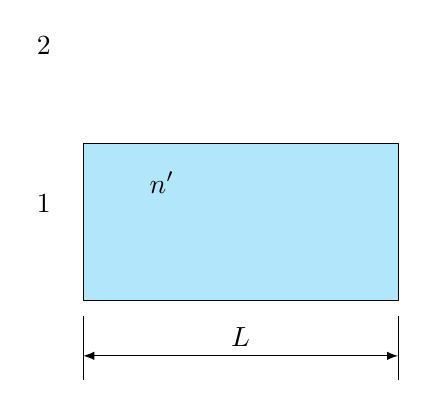
\begin{tikzpicture}[line cap=round,line join=round]
  \fill[cyan,opacity=0.3] (0,0) -- (0,2) -- (4,2) -- (4,0) -- cycle;
  \draw (0,0) -- (0,2) -- (4,2) -- (4,0) -- cycle;
  \ray(-1,3)(5,3)(0.5)(1);
  \ray(-1,1)(5,1)(0.5)(1);
  \draw (-0.5,1) node[above] {1};
  \draw (-0.5,3) node[above] {2};
  \draw (1,1.5) node[] {$n'$};
  \draw (0,-0.2) -- (0,-1);
  \draw (4,-0.2) -- (4,-1);
  \draw[latex-latex] (0,-0.7) -- (4,-0.7) node[above, pos=0.5] {$L$};
  \end{tikzpicture}
  \captionof{figure}{Problema \ref{p:PO205}\label{f:PO205}}
\end{center}
\end{minipage}
%
\begin{minipage}[c]{0.45\textwidth}
  \begin{center}
  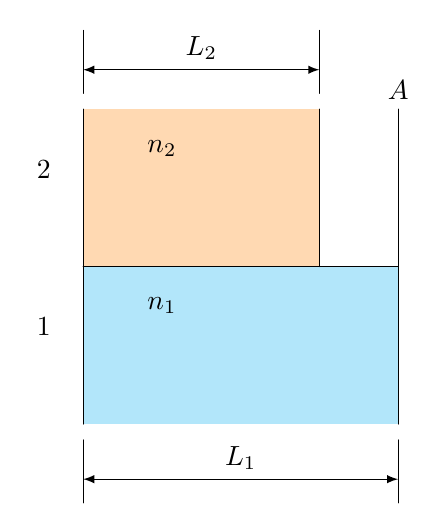
\begin{tikzpicture}[line cap=round,line join=round]
  \fill[cyan,opacity=0.3] (0,0) -- (0,2) -- (4,2) -- (4,0) -- cycle;
  \fill[orange,opacity=0.3] (0,2) -- (0,4) -- (3,4) -- (3,2) -- cycle;
  \draw (0,0) -- (0,4);
  \draw (0,2) -- (4,2);
  \draw (4,0) -- (4,4) node[above] {$A$};
  \draw (3,2) -- (3,4);
  \ray(-1,3)(5,3)(0.5)(1);
  \ray(-1,1)(5,1)(0.5)(1);
  \draw (-0.5,1) node[above] {1};
  \draw (-0.5,3) node[above] {2};
  \draw (1,1.5) node[] {$n_1$};
  \draw (1,3.5) node[] {$n_2$};
  \draw (0,4.2) -- (0,5);
  \draw (3,4.2) -- (3,5);
  \draw[latex-latex] (0,4.5) -- (3,4.5) node[above, pos=0.5] {$L_2$};
  \draw (0,-0.2) -- (0,-1);
  \draw (4,-0.2) -- (4,-1);
  \draw[latex-latex] (0,-0.7) -- (4,-0.7) node[above, pos=0.5] {$L_1$};
  \end{tikzpicture}
  \captionof{figure}{Problema \ref{p:PO202}\label{f:PO202}}
  \end{center}
\end{minipage}
%
\pma{\label{p:PO201}
En la figura \ref{f:PO201} se muestra el recorrido de dos haces de luz al reflejarse en superficies planas que están sumergidas en agua ($n = 1.3422$). Los haces tienen una longitud de onda en el vacío de $\SI{410}{nm}$ y están inicialmente en fase. \textit{a}) ¿Cuál es el valor mínimo de $L$ que hace que los haces estén en contrafase al salir de esa región? \textit{b}) ¿Y el segundo menor valor?
\rta{.90}{\textit{a}) $\SI{38.18}{nm}$; \textit{b}) $\SI{114.55}{nm}$}}
%
\begin{minipage}[c]{0.5\textwidth}
\begin{center}
  \begin{tikzpicture}[line cap=round,line join=round]
    \coordinate (C1)  at (0,0);
    \coordinate (C2)  at (0,1.5);
    \draw (-2,1.5) node[left] {Haz 2};
    \ray(-2,1.5)(C2)(0.5)(1);
    \ray(C2)(C1)(0.5)(1);
    \ray(C1)(2,0)(1)(1);
    \planemirror[cyan,opacity=0.2](C1)(1)(-45)(0.1);
    \planemirror[cyan,opacity=0.2](C2)(1)(135)(0.1);
    \draw[dashed] (-2,0) -- (-0.5,0);
    \draw[latex-latex] (-1.5,0) -- (-1.5,1.5) node[left, pos=0.5] {$L$};

    \coordinate (C3)  at (1.5,4.5);
    \coordinate (C4)  at (1.5,3);
    \coordinate (C5)  at (0,3);
    \coordinate (C6)  at (0,6);
    \draw (-2,4.5) node[left] {Haz 1};
    \ray(-2,4.5)(C3)(0.4)(1);
    \ray(C3)(C4)(0.5)(1);
    \ray(C5)(C6)(0.75)(1);
    \ray(C4)(C5)(0.5)(-1);
    \ray(C6)(2,6)(1)(1);
    \planemirror[cyan,opacity=0.2](C3)(1)(135)(0.1);
    \planemirror[cyan,opacity=0.2](C4)(1)(45)(0.1);
    \planemirror[cyan,opacity=0.2](C5)(1)(-45)(0.1);
    \planemirror[cyan,opacity=0.2](C6)(1)(225)(0.1);
    \draw[dashed] (-2,6) -- (-0.5,6);
    \draw[dashed] (-2,3) -- (-0.5,3);
    \draw[dashed] (0,6.2) -- (0,7);
    \draw[dashed] (1.5,6.2) -- (1.5,7);
    \draw[latex-latex] (-1.5,3) -- (-1.5,4.5) node[left, pos=0.5] {$L$};
    \draw[latex-latex] (-1.5,4.5) -- (-1.5,6) node[left, pos=0.5] {$L$};
    \draw[latex-latex] (0,6.6) -- (1.5,6.6) node[above, pos=0.5] {$L$};
  \end{tikzpicture}
  \captionof{figure}{Problema \ref{p:PO201}\label{f:PO201}}
\end{center}
\end{minipage}
%
\begin{minipage}[c]{0.5\textwidth}
  \begin{center}
  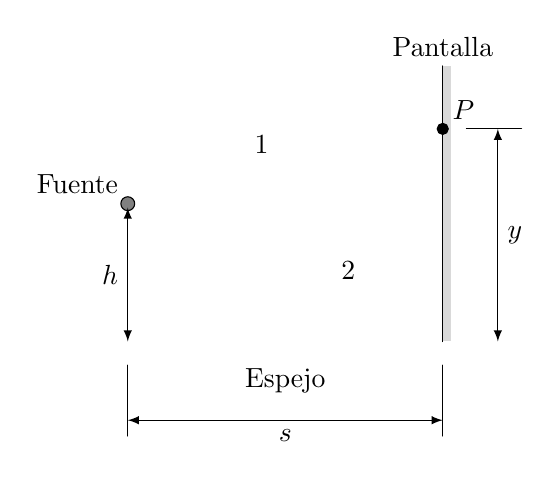
\begin{tikzpicture}[line cap=round,line join=round]
  \planemirror[cyan,opacity=0.2](0,0)(6)(0)(0.2);
  \fill[gray,opacity=0.3] (2,0) -- (2,3.5) -- (2.1,3.5) -- (2.1,0) -- cycle;
  \draw (2,0) -- (2,3.5) node[above] {Pantalla};
  \coordinate (F)  at (-2,1.75);
  \draw[fill=gray] (F) circle(2.5pt) node[above left] {Fuente};
  \draw[latex-latex] (-2,0) -- (-2,1.7) node[left, pos=0.5] {$h$};
  \draw (0,-0.5) node[] {Espejo};
  \draw[latex-latex] (-2,-1) -- (2,-1) node[below, pos=0.5] {$s$};
  \draw (-2,-0.3) -- (-2,-1.2);
  \draw (2,-0.3) -- (2,-1.2);
  \coordinate (P)  at (2,2.7);
  \filldraw[] (P) circle(2pt) node[above right] {$P$};
  \draw (P) + (0.3,0) --++ (1,0);
  \draw[latex-latex] (P) + (0.7,0) --++ (0.7,-2.7) node[right, pos=0.5] {$y$};
  \ray(F)(P)(0.5)(1);
  \coordinate (x) at (-0.455,0);
  \ray(x)(P)(0.5)(1);
  \ray(F)(x)(0.5)(1);
  \draw (-0.3,2.5) node[] {1};
  \draw (0.8,0.9) node[] {2};
  \end{tikzpicture}
  \captionof{figure}{Problema \ref{p:PO203}\label{f:PO203}}
  \end{center}
\end{minipage}
%
\pma{\label{p:PO203}
Determine el desfasaje entre los rayos 1 y 2 que llegan al punto $P$ (ver figura~\ref{f:PO203}) como función de su altura $y$ respecto del espejo. El sistema está inmerso en un medio de índice $n$.\\
\rta{.87}{$\Delta\phi=\frac{2\pi n}{\lambda_0} \left( \sqrt{(y+h)^2+s^2}-\sqrt{(y-h)^2+s^2} \right) \pm \pi $}}


% \pma{\label{p:PO204}
% Determine el desfasaje entre los rayos 1 y 2 que llegan al punto $P$ en el dispositivo de la figura \ref{f:PO204}. El material que atraviesa el rayo 1 tiene un índice de refracción $n'$ y el sistema está inmerso en un medio de índice de refracción $n$.\\
% \rta{.75}{$\Delta\phi=\frac{2\pi}{\lambda_0}\left(n\sqrt{4h^2+s^2}-n(s-d)-n' d\right) \pm \pi$}}
%
% \begin{center}
%   \begin{tikzpicture}[line cap=round,line join=round]
%   \planemirror[cyan,opacity=0.2](0,0)(6)(0)(0.2);
%   \fill[gray,opacity=0.3] (2,0) -- (2,3.5) -- (2.1,3.5) -- (2.1,0) -- cycle;
%   \draw (2,0) -- (2,3.5) node[above] {Pantalla};
%   \coordinate (F)  at (-2,1.75);
%   \draw[fill=gray] (F) circle(2.5pt) node[above left] {Fuente};
%   \draw[latex-latex] (-2,0) -- (-2,1.7) node[left, pos=0.5] {$h$};
%   \draw (0,-0.5) node[] {Espejo};
%   \draw[latex-latex] (-2,-1) -- (2,-1) node[below, pos=0.5] {$s$};
%   \draw (-2,-0.3) -- (-2,-1.2);
%   \draw (2,-0.3) -- (2,-1.2);
%   \coordinate (P)  at (2,1.75);
%   \filldraw[] (P) circle(2pt) node[above right] {$P$};
%   \draw (P) + (0.3,0) --++ (1,0);
%   \draw[latex-latex] (P) + (0.7,0) --++ (0.7,-1.75) node[right, pos=0.5] {$h$};
%   \fill[gray,opacity=0.3] (-0.5,2.2) -- (0.5,2.2) -- (0.5,1.3) -- (-0.5,1.3) -- cycle;
%   \draw[] (-0.5,2.2) -- (0.5,2.2) -- (0.5,1.3) -- (-0.5,1.3) -- cycle;
%   \draw (0,1.75) node[] {$n'$};
%   \ray(F)(-0.5,1.75)(0.5)(1);
%   \ray(0.5,1.75)(P)(0.5)(1);

%   \coordinate (x) at (0,0);
%   \ray(x)(P)(0.5)(1);
%   \ray(F)(x)(0.5)(1);
%   \draw (1,2) node[] {1};
%   \draw (1,0.5) node[] {2};
%   \draw (-0.5,2.4) -- (-0.5,3);
%   \draw (0.5,2.4) -- (0.5,3);
%   \draw[latex-latex] (-0.5,2.8) -- (0.5,2.8) node[above, pos=0.5] {$d$};
% \end{tikzpicture}
% \captionof{figure}{Problema \ref{p:PO204}\label{f:PO204}}
% \end{center}



